\documentclass{article}

% Recommended, but optional, packages for figures and better typesetting:
\usepackage{microtype}
\usepackage{graphicx}
\usepackage{subcaption}
\usepackage{booktabs} % for professional tables
\usepackage{dsfont}
% hyperref makes hyperlinks in the resulting PDF.
% If your build breaks (sometimes temporarily if a hyperlink spans a page)
% please comment out the following usepackage line and replace
% \usepackage{icml2026} with \usepackage[nohyperref]{icml2026} above.
\usepackage{hyperref}
\usepackage{multirow}
\usepackage[compact]{titlesec}
\usepackage[table]{xcolor}
\usepackage{array}
\usepackage{bm}

% Attempt to make hyperref and algorithmic work together better:
\newcommand{\theHalgorithm}{\arabic{algorithm}}

% Use the following line for the initial blind version submitted for review:
\usepackage{icml2026}

% For preprint, use
% \usepackage[preprint]{icml2026}

% If accepted, instead use the following line for the camera-ready submission:
% \usepackage[accepted]{icml2026}

\usepackage{amsmath}
\usepackage{amssymb}
\usepackage{mathtools}
\usepackage{amsthm}

% if you use cleveref..
\usepackage[capitalize,noabbrev]{cleveref}

% THEOREMS
\theoremstyle{plain}
\newtheorem{theorem}{Theorem}[section]
\newtheorem{proposition}[theorem]{Proposition}
\newtheorem{lemma}[theorem]{Lemma}
\newtheorem{corollary}[theorem]{Corollary}
\theoremstyle{definition}
\newtheorem{definition}[theorem]{Definition}
\newtheorem{assumption}[theorem]{Assumption}
\theoremstyle{remark}
\newtheorem{remark}[theorem]{Remark}

% Todonotes is useful during development; simply uncomment the next line
%    and comment out the line below the next line to turn off comments
%\usepackage[disable,textsize=tiny]{todonotes}
\usepackage[textsize=tiny]{todonotes}

% The \icmltitle you define below is probably too long as a header.
% Therefore, a short form for the running title is supplied here:
\icmltitlerunning{Diffusion Language Models Are Natively Length-Aware}

\begin{document}

\twocolumn[
  \icmltitle{Diffusion Language Models Are Natively Length-Aware}

  % It is OKAY to include author information, even for blind submissions: the
  % style file will automatically remove it for you unless you've provided
  % the [accepted] option to the icml2026 package.

  % List of affiliations: The first argument should be a (short) identifier you
  % will use later to specify author affiliations Academic affiliations
  % should list Department, University, City, Region, Country Industry
  % affiliations should list Company, City, Region, Country

  % You can specify symbols, otherwise they are numbered in order. Ideally, you
  % should not use this facility. Affiliations will be numbered in order of
  % appearance and this is the preferred way.
  \icmlsetsymbol{equal}{*}

  \begin{icmlauthorlist}
    \icmlauthor{Vittorio Rossi}{equal,yyy}
    \icmlauthor{Giacomo Cirò}{equal,yyy}
    \icmlauthor{Davide Beltrame}{equal,yyy}
    \icmlauthor{Luca Gandolfi}{yyy}
    \icmlauthor{Paul Röttger}{yyy}
    \icmlauthor{Dirk Hovy}{yyy}
  \end{icmlauthorlist}

  \icmlaffiliation{yyy}{Department of Computing Sciences, Bocconi University, Milan, Italy}

  \icmlcorrespondingauthor{Dirk Hovy}{dirk.hovy@unibocconi.it}

  % You may provide any keywords that you find helpful for describing your
  % paper; these are used to populate the "keywords" metadata in the PDF but
  % will not be shown in the document
  \icmlkeywords{Machine Learning, ICML, Diffusion language models, Inference, Speedup, Model properties}

  \vskip 0.3in
]

% this must go after the closing bracket ] following \twocolumn[ ...

% This command actually creates the footnote in the first column listing the
% affiliations and the copyright notice. The command takes one argument, which
% is text to display at the start of the footnote. The \icmlEqualContribution
% command is standard text for equal contribution. Remove it (just {}) if you
% do not need this facility.

% Use ONE of the following lines. DO NOT remove the command.
% If you have no special notice, KEEP empty braces:
% \printAffiliationsAndNotice{}  % no special notice (required even if empty)
% Or, if applicable, use the standard equal contribution text:
\printAffiliationsAndNotice{\icmlEqualContribution}

\begin{abstract}
Unlike autoregressive language models, which terminate variable-length generation upon predicting an End-of-Sequence (\verb|EoS|) token, Diffusion Language Models (DLMs) operate over a fixed maximum-length context window for a predetermined number of denoising steps. However, this process is independent of the required response length, resulting in computational waste for the majority of short responses common in reasoning and chat tasks.
To address this problem, we conjecture that the latent prompt representation contains sufficient information to estimate the required output length. We provide empirical evidence for this phenomenon and propose a zero-shot mechanism to dynamically crop the context window before generation begins, leading to fewer diffusion steps and substantial computational savings.
We evaluate our approach on four benchmarks with diverse tasks---\verb|GSM8K| (reasoning), \verb|HumanEval| (code generation), \verb|IfEval| (instruction following), and \verb|LongFormQA| (question answering)---revealing massive efficiency gains at minimal performance impact. We report significant reductions in FLOPs across all tasks, with no statistically significant performance degradation, and significant performance improvements in 2 out of 4 tasks.
\end{abstract}

% FROM THE MEETING ON 2026-01-15:
% the paper as written so far seems fine, however we’re two pages under the limit: we could add a deeper motivation into the performance improvement
% benefit is larger for shorter answers, should we elaborate on this?
% problem is existence of ground truth: it’s fine to associate the outcome of the model with the intermediate result of the same model
% performance is not driven by absolute length but this is fine because we’re looking at relative savings
% we need to make clear in table1 what the baseline we choose is and what the avg predicted length is
% we could’ve fixed a maximum context length to compare it as a bound of the predicted context length
% plotting table 1 performance to show confidence intervals might duplicate information, whereas length prediction analysis is more needed
% we can bucket for each data set predicted response length and performance in a histogram. we expect a clean curve, descriptive but useful visual result

% FROM THE MEETING ON 2026-01-23:
% specify confidence intervals through bootstrapping, despite not actual significance testing
% in a footnote: we initially explored modernbert for diffusion, etc.; if we only test one model the significance testing is crucial to make people understand that the observed effect will generalize across datasets pretty confidently ;
% rho or pi for the prompt, there are three different p’s. notation has to be crystal clear

\section{Introduction}
\label{sec:intro}
Language generation with Large Language Models (LLMs) has been dominated by autoregressive models, which generate text sequentially, predicting one token at a time~\cite{Zou2023}. While proven successful, this sequential mechanism inherently limits inference speed and brings various disadvantages, such as the inability to perform global refinements during the generation process and error propagation due to ``wrong'' early tokens. Recently, Diffusion Language Models ~\citep[DLMs,][]{Austin2021D3PM, lou2024discretediffusionmodelingestimating} have emerged as a promising alternative, offering the potential for accelerated, non-autoregressive generation through iterative denoising
\begin{figure}
    \centering
    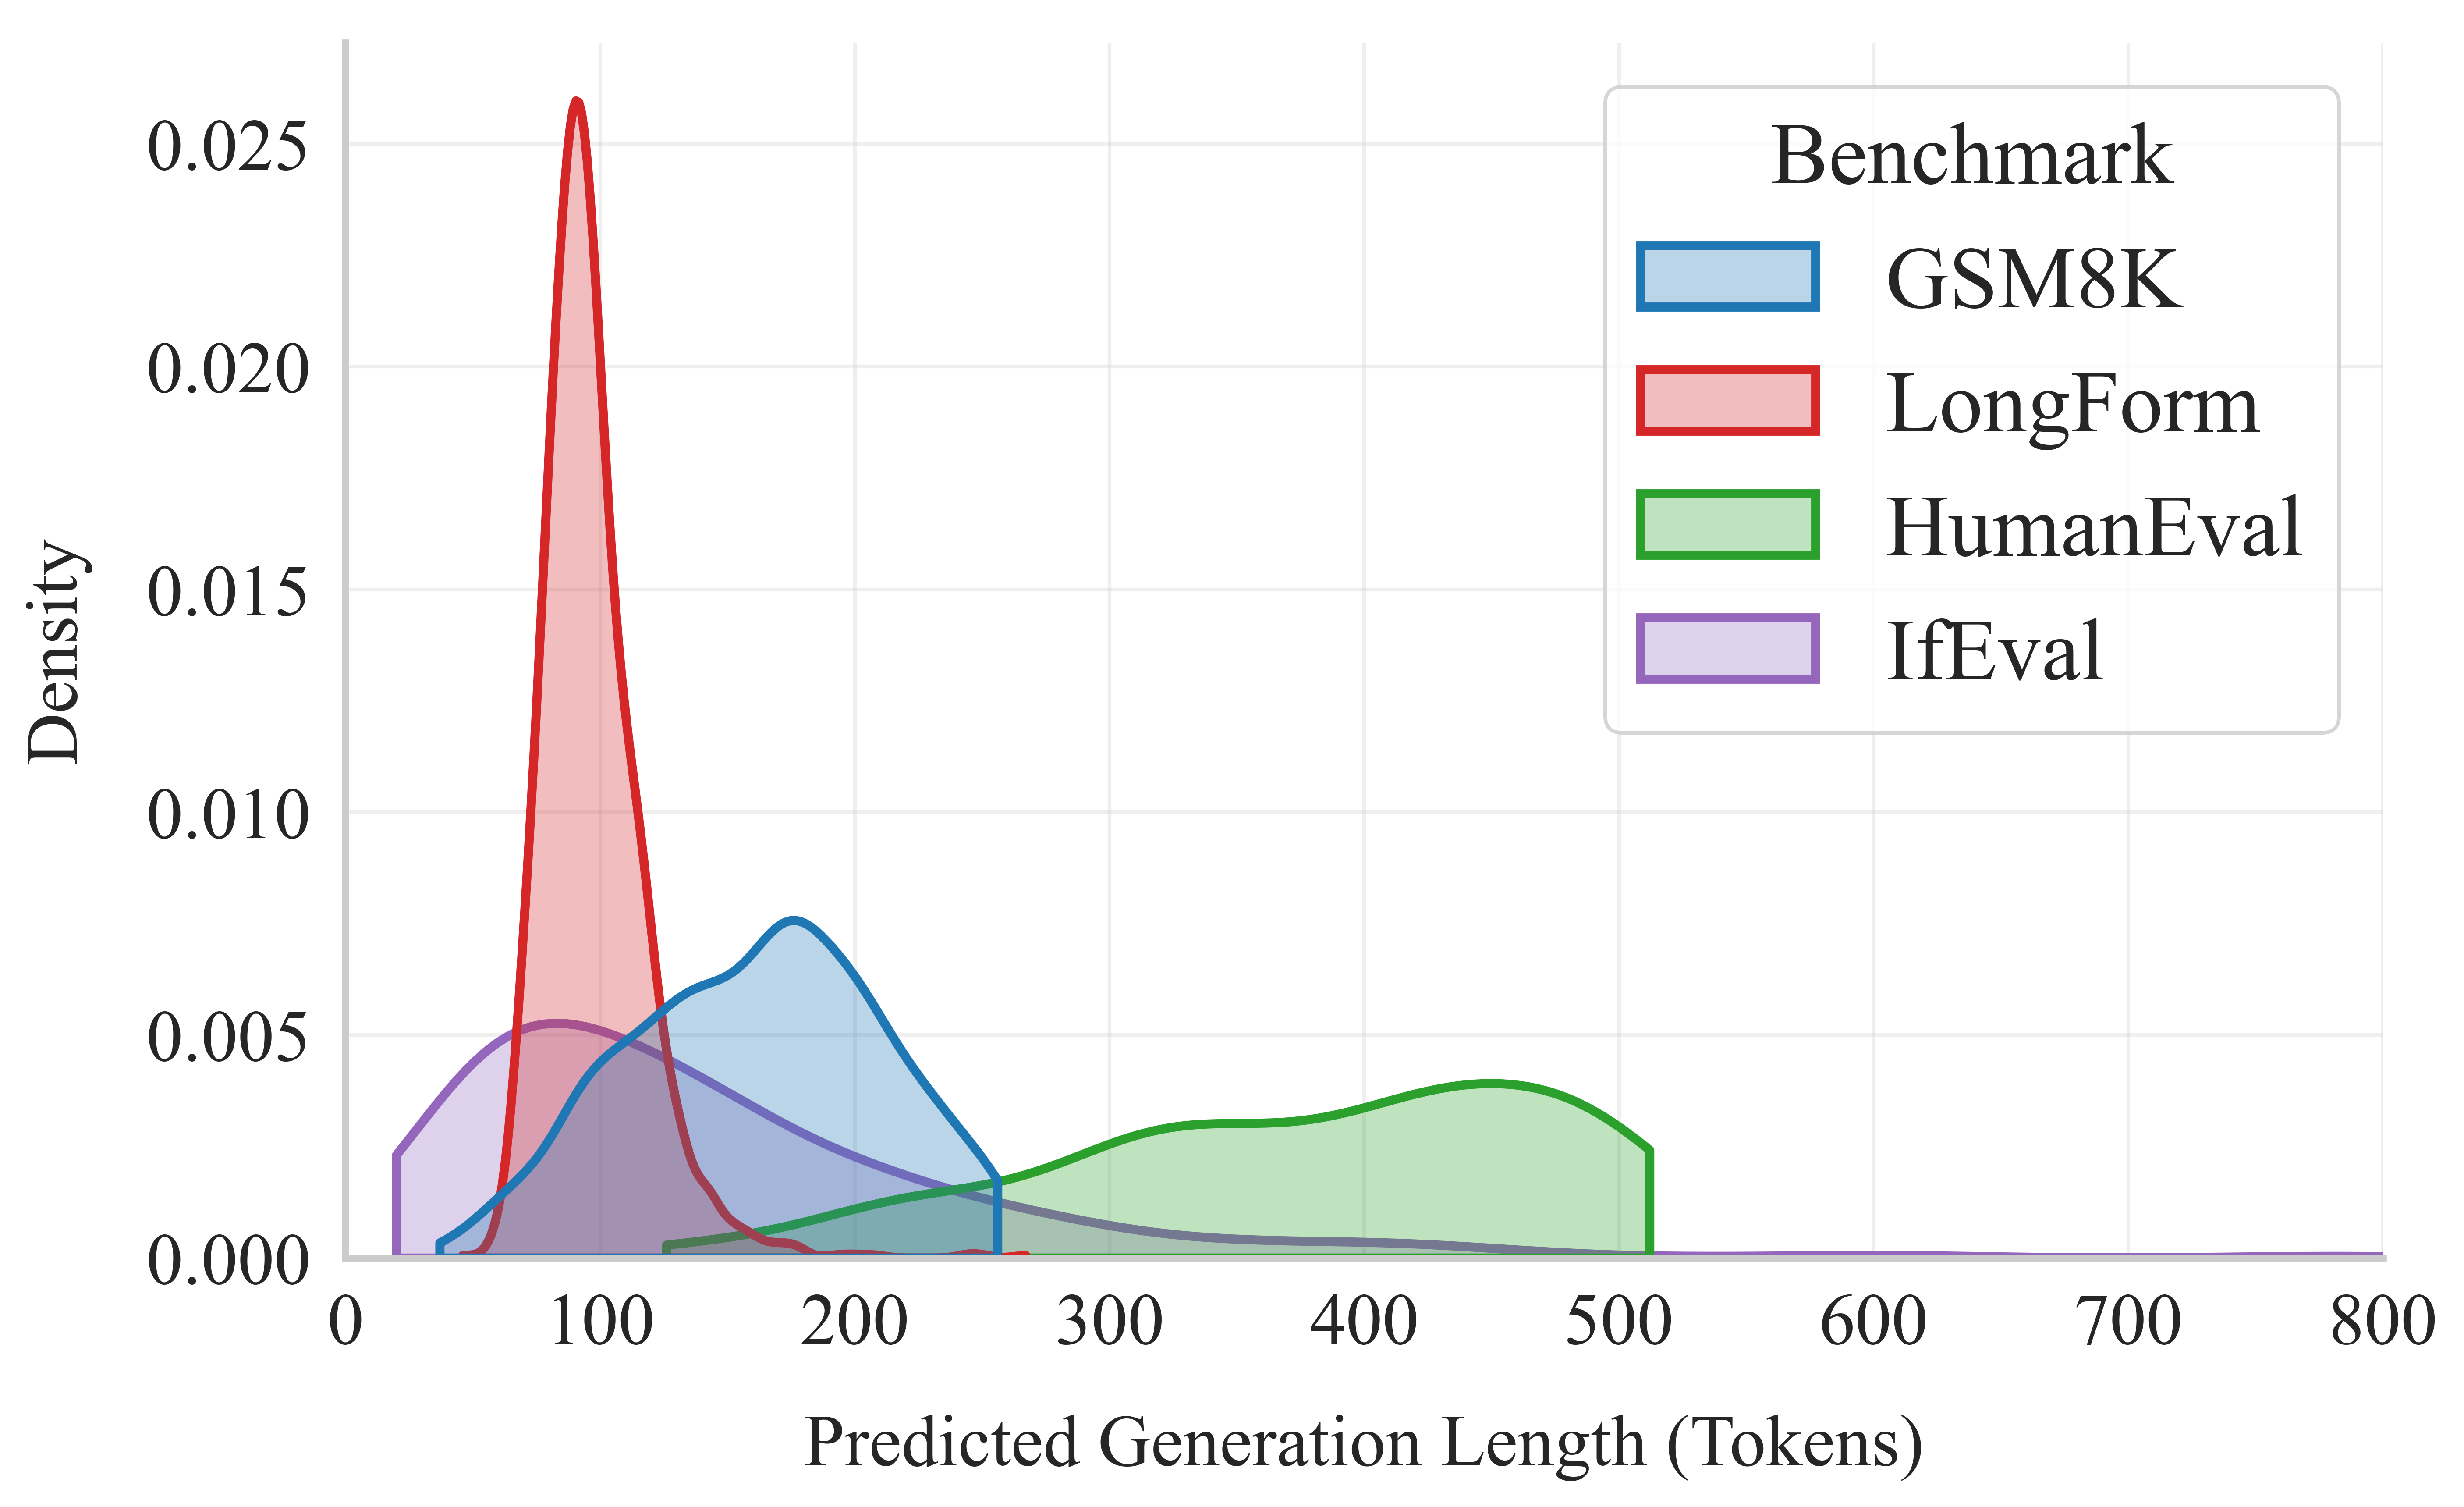
\includegraphics[width=\linewidth]{img/hero.png}
    \caption{\textbf{Predicted Length Distributions.}
    Our \textsc{SmartCrop} ($\tau = 0.9$) method successfully predicts task-specific output lengths across four benchmark datasets. The abrupt truncations observed in certain distributions correspond to context length constraints (refer to Section~\ref{sec:experiments} for details).}
    \label{fig:distributions}
\end{figure}
DLMs operate by progressively unmasking tokens on a fixed-length canvas. This process is initialized with a prompt, while the remainder of the maximum context window is filled with placeholder mask tokens. In each denoising step, the model predicts logits for the entire masked sequence and unmasks a subset of tokens, typically those with the highest confidence. Unmasked tokens are kept and the process repeated. While this allows for flexible, parallel sequence generation, the requirement of a fixed canvas length remains a significant bottleneck, as the dimensions must be defined \textit{a priori} based on heuristics or domain knowledge. To support variable-length outputs, current approaches often rely on padding with special End-of-Sequence (\verb|EoS|) tokens to prevent unmasking beyond a certain point~\cite{nie2025large}. However, this introduces substantial computational waste: the model must still process the entire context window during every forward pass, regardless of the actual output length

In this work, we conjecture that DLMs implicitly encode the required output length within their latent representation of the prompt. In other words, DLMs encode an expectation about how many answer tokens are needed, depending on the task or question they are prompted with. While these models 
are explicitly trained to predict EoS tokens at appropriate positions, 
we show that this length signal can be extracted and exploited *before* 
generation begins, rather than discovered iteratively during denoising

Building on this, we introduce \textsc{SmartCrop}, a model-native method to optimize DLM inference. We transform \verb|EoS| logits into a cumulative ``inverse survival" probability across positions, modeling the likelihood of the response terminating at any given point on the canvas. By identifying the first position where this probability exceeds a specified threshold (e.g., $\tau = 0.9$), we dynamically crop the canvas before generation begins. We then run the standard denoising schedule on the new, shorter canvas.

We evaluate our approach using \texttt{LLaDa}~\cite{nie2025large}, a state-of-the-art 8 billion parameters DLM trained to handle variable-length outputs via \verb|EoS| padding, and test it on four benchmarks with a diverse range of tasks: \texttt{GSM8K} \citep[reasoning,][]{cobbe2021trainingverifierssolvemath}, \texttt{HumanEval} \citep[code generation,][]{chen2021evaluatinglargelanguagemodels}, \texttt{IfEval} \citep[instruction following,][]{zhou2023instructionfollowingevaluationlargelanguage}, and \texttt{LongFormQA} \citep[question answering][]{koksal2023longform}. 

Our results demonstrate that \textsc{SmartCrop} drastically reduces computational costs, measured in FLOPs, with negligible impact on performance. Notably, we observe no statistically significant performance degradation across any benchmark and significant performance improvements in 2 of the 4 evaluation suites. These findings suggest that DLMs trained with the \verb|EoS| paradigm are inherently ``length-aware", and that \textsc{SmartCrop} effectively leverages this previously unobserved behavior to bridge the efficiency gap between fixed-canvas diffusion and variable-length generation.

We make our code and results publicly available on GitHub.\footnote{\url{na}.}

% The magnitude of these efficiency gains strongly depends on the `slack' in the baseline context window (C). When generating, users must choose a conservative, large C to avoid truncating long outlier responses, forcing the model to pay a high compute cost for every prompt. Another advantage of \textsc{SmartCrop} is that it eliminates this necessity. 
% For GSM8K and HumanEval, we used the tight context lengths optimized by the \citep[LLaDa][]{yang2025diffusionllmnativevariable} authors, leaving naturally little 'slack' for our method to remove. For IfEval, we adopted the 1280-token window from the \citep[Dream][]{ye2025dream7bdiffusionlarge} paper to simulate a realistic `safe' buffer; this allowed us to test the mechanism with significant slack, where \textsc{SmartCrop} yielded massive speedups ($>$90\%) by pruning the excess capacity. Finally, for LongFormQA, we established a baseline of 512 tokens and 64 denoising steps to specifically evaluate performance in multi-unmask scenarios. This demonstrates that SmartCrop effectively automates context-length optimization, providing the largest benefits in the most realistic scenarios where C is set conservatively high.

\section{Related Work}
\label{sec:related_work}

\paragraph{Diffusion models for text.}
Diffusion models originate from non-equilibrium thermodynamics and were first developed for continuous data~\citep{SohlDickstein2015,Ho2020DDPM}.
Several works adapt diffusion to discrete text.
Structured Denoising Diffusion Models in Discrete State-Spaces (D3PM) define masked corruption processes for tokens and show that discrete diffusion can serve as a general generative framework~\citep{Austin2021D3PM}.
Diffusion-LM applies diffusion in the embedding space and improves controllable text generation~\citep{Li2022DiffusionLM}.
DiffuSeq extends this idea to sequence-to-sequence tasks~\citep{Gong2022DiffuSeq}, and DiffusionBERT integrates diffusion training with pre-trained masked language models~\citep{He2022}.
Lou et al.\ model discrete diffusion by estimating ratios of the data distribution and obtain strong likelihood estimates~\citep{lou2024discretediffusionmodelingestimating}.
Zou et al.\ survey this growing line of work under the umbrella term diffusion language models~\citep{Zou2023}.

\paragraph{Scaling.} Recent work scales masked diffusion models (MDMs) to the LLM regime (DLLMs).
Gong et al.\ adapt large autoregressive transformers into diffusion models and study how performance scales with model size~\citep{Gong2025}.
Liang et al.\ derive scaling laws for diffusion transformers and analyze compute--performance trade-offs~\citep{Liang2024}.
LLaDA trains a large diffusion language model from scratch and shows that it can match autoregressive LLMs on instruction-following and reasoning benchmarks~\citep{nie2025large}.
These works demonstrate that DLLMs are competitive with autoregressive models, but they still rely on fixed-length diffusion canvases at inference time.

\paragraph{Efficiency and sampling.} Several methods improve the sampling efficiency of diffusion models. Early work in vision reduces the number of denoising steps while maintaining sample quality~\citep{Ho2020DDPM}.
In text, DiffusionBERT reports that diffusion-style objectives can reuse pre-trained encoders and achieve strong generation quality with moderate sampling cost~\citep{He2022}.
Other work studies the trade-offs of non-autoregressive generation more broadly~\citep{DBLP:journals/corr/abs-2004-10454}.
These approaches make each denoising trajectory cheaper, but they keep the sequence length fixed and do not address the padding tax caused by short outputs.
Block Diffusion instead interpolates between autoregressive and diffusion decoding~\citep{Arriola2025}.
It decodes overlapping blocks of tokens and can reduce latency for long sequences.
However, it sacrifices some of the full-sequence parallelism that makes MDMs attractive and still relies on a predetermined maximum context length.

\paragraph{Variable-length generation.} A more recent line of work aims to remove the fixed-canvas constraint.
DAEDAL proposes a training-free method that dynamically adjusts the canvas length during sampling~\citep{li2025fixedtrainingfreevariablelengthdenoising}.
It starts from a short canvas, uses internal confidence scores to decide when to expand, and inserts additional masked tokens when parts of the sequence look under-developed.
This strategy increases the fraction of useful tokens but requires several rounds of expansion and custom heuristics.

Yang et al.\ introduce a diffusion LLM with native variable generation lengths (dLLM-Var)~\citep{yang2025diffusionllmnativevariable}.
They modify training so that the model predicts \texttt{EoS} more accurately and support blockwise diffusion guided byn\texttt{EoS} detection. At inference time, dLLM-Var can stop denoising when \texttt{EoS} is predicted with high confidence, without relying on a fixed context. This approach delivers large speedups but requires retraining with new objectives and specialized decoding.

Our work sits between these extremes.
Like DAEDAL, we use a training-free method on top of existing scaled MDMs.
Like dLLM-Var, we rely on \texttt{EoS} behavior.
However, we do not expand or modify the canvas during denoising and we do not change training.
Instead, we show that a single early denoising step already encodes a useful distribution over output length, and we exploit it to crop the canvas once before standard diffusion decoding.

\paragraph{Length control in other LMs.} Non-autoregressive sequence models often predict output length explicitly or learn to stop decoding based on special tokens~\citep{DBLP:journals/corr/abs-2004-10454}.
Su et al.\ propose BERT-CRF for non-autoregressive text generation with dynamic output length~\citep{Gu2021BERTCRF}.
Kaneko and Okazaki reduce sequence length by predicting edit operations that remove redundant tokens~\citep{kaneko2023reducingsequencelengthpredicting}.
These works confirm that internal representations can carry strong signals about the eventual output length and structure.

Distillation and model compression reduce computational cost~\citep{Sanh2019DistilBERT}, and early exiting has been explored in other settings.
In contrast, our method targets diffusion-style decoding and uses an inverse survival function over \texttt{EoS} logits to decide how much of the canvas to keep before sampling.

\section{Methodology}
\label{sec:methodology}

Let $V$ denote the vocabulary size, $L_p$ the length of the tokenized prompt, and $L_c$ the fixed context window size of the model. At the initialization of the generation process, a DLM receives an input sequence $\mathbf{x}$, constructed by concatenating the raw tokenized prompt $\mathbf{x}_{\text{prompt}}=(x_1, \dots,x_{L_p})\in\{0,1, \dots, V-1\}^L_p$ with a sufficient number of placeholder \texttt{<mask>} tokens to fill the context length $L_c$:
\begin{equation}
\mathbf{x}=(\mathbf{x}_{\text{prompt}}, \underbrace{\texttt{<mask>}, \dots, \texttt{<mask>}}_{L_c-L_p\text{ times}})
\end{equation}

The model encodes this input into latent space and infers a probability distribution over the vocabulary for each masked position. Through iterative sampling, a subset of \texttt{<mask>} tokens is replaced (unmasked) at each step, and the process repeats until the sequence is fully generated. To support variable-length generation within this fixed-length paradigm, a special end-of-sentence token (\texttt{EoS}) is included in the vocabulary. The model learns to use \texttt{EoS} as a padding token for positions exceeding the meaningful output length. However, this architectural constraint forces the model to process the full context window of length $L_c$ during every forward pass, incurring significant and often unnecessary computational costs.

We hypothesize that during pre-training, the model learns to encode information regarding the required output length within the latent representation of the initial input. We propose to extract this signal to perform dynamic context truncation.

Let $L^*$ be a random variable representing the true output length. We want to estimate the cumulative probability that the generation terminates at position $\ell$, i.e., $\Pr(L^* \le \ell)$ for any $\ell \in \{L_p+1, \dots, L_c\}$. By applying a softmax function to the model's logits, we obtain the local probability $\phi_{i} = \Pr(\text{token}_i = \texttt{EoS})$ for each position $i$. Consequently, the probability that the sequence has \emph{not} ended by position $\ell$ is the joint probability of not observing an \texttt{EoS} token at any position from $L_p+1$ to $\ell$. Therefore, the cumulative probability of the sequence ending at or before $\ell$ is given by:
\begin{equation}
\Pr(L^* \le \ell) = 1 - \prod_{j=L_p+1}^{\ell} (1 - \phi_j)
\end{equation}

Using this cumulative distribution, we determine the predicted length $\hat{L}$ as the minimal position where this probability exceeds a predefined confidence threshold $\tau\in[0,1]$:
\begin{equation}
\hat{L} = \min \{ \ell \in \{L_p+1, \dots, L_c\} \mid \Pr(L^* \le \ell) \ge \tau \}
\end{equation}

Upon determining $\hat{L}$, we truncate the initial context window by removing the final $L_c-\hat{L}$ \texttt{<mask>} tokens. This ensures that for all subsequent denoising steps, the model processes a reduced context window of size $\hat{L}$.

This method serves as a lightweight, plug-and-play optimization applied immediately after the initial forward pass, significantly reducing the computational burden for the remainder of the generation process.

\section{Experiments}
\label{sec:experiments}
%\begin{itemize}
%    \item talk about the ablation tests we do (predict random mean)
%    \item talk about benchmark-specific distribution
%\end{itemize}

% We evaluate \textsc{SmartCrop} decoding on \texttt{LLaDa} 8B Instruct model and four benchmarks.
% Our experiments answer three questions.
% First, how much computation does \textsc{SmartCrop} save relative to fixed-length decoding?
% Second, how sensitive generation quality is to length mis-estimation?
% Third, what kind of length information does the model encode at the initial denoising step?

\subsection{Models}

Our experiments utilize \texttt{LLaDA}~\citep{nie2025large}, a state-of-the-art 8 billion parameters DLM. It implements a masked denoising protocol within a fixed context window during baseline decoding and supports variable-length generation through the \texttt{EoS}-as-padding paradigm. Our evaluation focuses on this model as it is currently the only open-source, high-performance native DLM that incorporates this \texttt{EoS} capability.

While we also considered \texttt{ModernBERT}~\citep{dllm} adapted for diffusion generation, the relatively small model scale and limited performance yielded inconclusive results. Consequently, we focus our analysis solely on \texttt{LLaDA}, as its architecture and training objective provide the most robust environment for evaluating ``length-aware" behaviors in large-scale DLMs.
We emphasize that \textsc{SmartCrop} is designed specifically for EoS-trained diffusion models and makes no claims about DLMs trained with alternative paradigms.


\subsection{Benchmarks}

We evaluate our proposed \textsc{SmartCrop} method against baseline decoding across four capability benchmarks selected to span distinct output-length regimes. Although text generation tasks generally lack an explicit ground-truth length, this selection allows us to investigate length-prediction behavior across qualitatively different domains. As illustrated in Fig.~\ref{fig:distributions}, our method successfully recovers task-specific length distributions from the latent prompt representations.

To maintain consistency with established literature while exploring the limits of diffusion efficiency, we define specific context lengths ($L_c$) and denoising schedules ($T$) for each task (Table~\ref{tab:benchmarks}).

\paragraph{Mathematical Reasoning} \texttt{GSM8K} targets structured, short-form reasoning \citep{cobbe2021trainingverifierssolvemath}. Following \citet{nie2025large}, we set $L_c=256$ tokens. Performance is measured via \textit{Exact-Match Accuracy}, verifying if the final numerical output aligns with the ground truth.

\paragraph{Code Generation} \texttt{HumanEval} evaluates functional correctness \citep{chen2021evaluatinglargelanguagemodels}. We utilize $L_c=512$ tokens, consistent with the original \texttt{LLaDA} evaluation. Performance is measured using \textit{Pass@1}, which assesses the functional correctness of generated code via unit tests.

\paragraph{Instruction Following} \texttt{IfEval} assesses adherence to objective constraints \citep{zhou2023instructionfollowingevaluationlargelanguage}. We set the context length to $L_c=1280$ tokens, following the experimental setup in \citet{ye2025dream7bdiffusionlarge}. This expanded window provides a testbed for our method’s ability to achieve significant token savings. Performance is measured by \textit{Strict Accuracy}, a prompt-level metric verifying if the response satisfies all specified constraints (e.g., formatting, word counts).

\paragraph{Question Answering} \texttt{LongFormQA} evaluates free-form answering \citep{koksal2023longform} and represents a realistic chat-based scenario. Performance is measured using \textit{ROUGE-1}, quantifying the unigram overlap between the generation and the reference answer. We acknowledge that performance on this benchmark is sensitive to the metric’s inherent dependence on total sequence length.

Given computational constraints, we adopted a focused parameter selection rather than an exhaustive grid search. For \texttt{GSM8K}, \texttt{HumanEval}, and \texttt{IfEval}, the number of denoising steps is set equal to the context length ($T=L_c$) to establish a high-fidelity baseline. For \texttt{LongFormQA}, we fix the denoising schedule to $T=64$ steps. This allows us to evaluate \textsc{SmartCrop} in a high-density generation regime, where the model must predict multiple tokens per step.

\begin{table}[t]
\centering
% \resizebox forces the table to occupy exactly the width of the column
\resizebox{\columnwidth}{!}{%
\begin{small}
\begin{tabular}{lccc}
\hline 
\textbf{Benchmark} & \textbf{Context ($L_c$)} & \textbf{Steps ($T$)} & \textbf{Content} \\
\hline 
\texttt{GSM8K} & 256 & 256 & Math \\
\texttt{HumanEval} & 512 & 512 & Code \\
\texttt{IfEval} & 1280 & 1280 & Instruction \\
\texttt{LongFormQA} & 512 & 64 & QA \\
\hline 
\end{tabular}
\end{small}
}
\caption{\textbf{Experimental Configurations.} Summary of hyper-parameters across benchmark datasets. \textit{Context} ($L_c$) denotes the fixed canvas length (in tokens) utilized during the initial forward pass, inclusive of the prompt tokens. \textit{Steps} ($T$) indicates the total number of denoising iterations. For example, $L_c=256$ with $T=256$ implies a linear schedule where exactly 1 token is unmasked per step (the effective number of tokens to be unmasked is $L_c-L_p$, where $L_p$ is the prompt length). \textit{Content} describes the task domains represented in each dataset.}
\label{tab:benchmarks}
\end{table}

\subsection{Baselines}

To validate our length estimation hypothesis, we compare two distinct decoding strategies.

\paragraph{Full Context.} This serves as the standard diffusion baseline, where the model denoises a fixed-length context window of size $L_c$ for all prompts.

\paragraph{\textsc{SmartCrop} (Ours).} Our proposed mechanism dynamically adjusts the generation canvas. We perform a single forward pass at the initial denoising step and convert the \texttt{EoS} logits into a cumulative probability distribution over positions. The canvas is cropped at the smallest position where the cumulative probability exceeds a threshold $\tau$ (default $\tau = 0.9$). Subsequent denoising steps are then executed exclusively on this reduced window.

We quantify computational efficiency using total floating-point operations (FLOPs) and report relative reductions compared to the \textit{Full Context} baseline. Performance comparisons between the decoding strategies are detailed in Table \ref{tab:main_results}.

\subsection{Sensitivity Analysis}

To evaluate the robustness of our length prediction $\hat{L}$, we perform a sensitivity analysis by perturbing the cropped window size. We modulate the effective context length by applying a deviation factor $\delta \in [-50\%, +50\%]$ to the predicted length $\hat{L}$, defined as:
\begin{equation}
    \ell_{\delta} = \hat{L} \cdot (1 + \delta).
\end{equation}
By sweeping $\delta$ in 10\% increments, we observe the sensitivity of model performance to the allocated sequence length. This controlled perturbation allows us to discern whether the efficiency gains stem from the model's ability to identify a precise, prompt-specific bound, or if they are merely a byproduct of reducing a generic, oversized context.

Furthermore, to isolate the effect of task-specific length estimation, we introduce a stochastic control. We compare our method against a baseline where the context length is sampled at random from the aggregate distribution of predicted lengths across the other benchmarks. This comparison serves to confirm that the observed performance is due to instance-specific predictions rather than a broad, task-agnostic reduction in sequence length.

We conduct this analysis on the \texttt{IfEval} benchmark, as its generous maximum context window ($L_c$) provides a sufficiently wide range for meaningful observation. The results, illustrated in Fig.~\ref{fig:quality_sweep}, demonstrate how model performance scales as the context window converges toward or diverges from our predicted optimum.

\section{Results}
\label{sec:results}

\begin{table*}[t]
\centering
\small
\caption{\textbf{Main Results.} Performance comparison between native diffusion decoding and our proposed dynamic cropping method across four benchmarks using the \texttt{LLaDA} architecture. 
\textit{Benchmark} indicates the evaluation suite.
\textit{Method} distinguishes between the native Full Context (\textsc{FC}) baseline and our \textsc{SmartCrop} (\textsc{SC}) approach at various length-prediction quantiles ($\tau$). 
\textit{Avg. Tokens} represents the mean sequence length of the generated output, including the prompt prefix. 
\textit{Metric} denotes the task-specific performance score, where $^*, ^{**},$ and $^{***}$ indicate statistical significance at the $p < 0.05, 0.01,$ and $0.001$ levels, respectively. 
\textit{FLOPs Saved} quantifies the reduction in total floating-point operations relative to the \textsc{FC} baseline (e.g., a 98\% saving implies our method requires only 2\% of the baseline computation). 
\textit{Perf. $\Delta$} reports the relative percentage change in performance compared to the \textsc{FC} baseline.
}
\label{tab:main_results}
\setlength{\tabcolsep}{6pt}
\centering
\begin{tabular}{llc|ccc}
\toprule
\textbf{Benchmark} & \textbf{Method} & \textbf{Avg Tokens} & \textbf{Metric} & \textbf{FLOPs Saved${(\%)}$} & \textbf{Perf.${\Delta(\%)}$} \\
\midrule
\multirow{6}{*}{\textbf{IfEval}} & FC & 1280.0 & $0.4801$ & - & - \\
 & \textsc{SC-0.5} & 112.5 & $0.5342^{*}$ & 98.47\% & +11.25\% \\
 & \textsc{SC-0.75} & 129.5 & $0.5521^{**}$ & 98.05\% & +14.99\% \\
 & \textsc{SC-0.9} & 144.4 & $0.5459^{**}$ & 97.64\% & +13.70\% \\
 & \textsc{SC-0.95} & 153.2 & $0.5450^{**}$ & 97.37\% & +13.50\% \\
 & \textsc{SC-0.99} & 167.3 & $\bm{0.5694}^{***}$ & 96.92\% & +18.58\% \\
\midrule
\multirow{6}{*}{\textbf{GSM8K}} & FC & 256.0 & $\bm{0.5616}$ & - & - \\
 & \textsc{SC-0.5} & 116.5 & $0.5452$ & 69.39\% & -2.92\% \\
 & \textsc{SC-0.75} & 141.5 & $0.5516$ & 59.09\% & -1.77\% \\
 & \textsc{SC-0.9} & 161.1 & $0.5457$ & 50.15\% & -2.83\% \\
 & \textsc{SC-0.95} & 171.9 & $0.5490$ & 44.93\% & -2.25\% \\
 & \textsc{SC-0.99} & 187.7 & $0.5520$ & 37.01\% & -1.71\% \\
\midrule
\multirow{6}{*}{\textbf{HumanEval}} & FC & 512.0 & $0.4592$ & - & - \\
 & \textsc{SC-0.5} & 341.8 & $0.4665$ & 46.42\% & +1.59\% \\
 & \textsc{SC-0.75} & 362.2 & $0.4688$ & 41.06\% & +2.08\% \\
 & \textsc{SC-0.9} & 378.9 & $\bm{0.4851}$ & 36.53\% & +5.65\% \\
 & \textsc{SC-0.95} & 388.2 & $0.4598$ & 33.98\% & +0.13\% \\
 & \textsc{SC-0.99} & 402.0 & $0.4106$ & 30.16\% & -10.59\% \\
 \midrule
 \multirow{6}{*}{\textbf{LongFormQA}} & FC & 512.0 & $0.1341$ & - & - \\
 & \textsc{SC-0.5} & 79.4 & $0.2115^{***}$ & 85.40\% & +57.72\% \\
 & \textsc{SC-0.75} & 88.8 & $0.2152^{***}$ & 82.56\% & +60.48\% \\
 & \textsc{SC-0.9} & 97.1 & $0.2173^{***}$ & 79.94\% & +62.01\% \\
 & \textsc{SC-0.95} & 102.1 & $0.2196^{***}$ & 78.35\% & +63.73\% \\
 & \textsc{SC-0.99} & 110.0 & $\bm{0.2210}^{***}$ & 75.86\% & +64.83\% \\
\bottomrule
\end{tabular}
\end{table*}


\subsection{\textsc{SmartCrop} Substantially Reduces Compute Cost}

\textsc{SmartCrop} consistently reduces the fraction of the masked canvas the model must denoise at each iteration, which directly translates into fewer token-position evaluations per step, thereby lowering the total FLOPs count. Across our benchmarks, \textsc{SmartCrop} reduces FLOPs by 46--98\% relative to full-context diffusion decoding, achieving an average computational saving of 67\%. The most substantial gains are observed in tasks requiring concise outputs, such as \verb|IfEval|, \verb|GSM8K|, and \verb|LongFormQA|. In these settings, the predicted length distribution concentrates around approximately 100--150 tokens. Consequently, cropping eliminates vast unused regions of the canvas. This is particularly evident in \verb|LongFormQA|, where we employ a longer initial canvas of 1,280 tokens. Even on \verb|HumanEval|, where the average output length ($374.62$ tokens) is closer to the initial context size ($512$ tokens), the method yields compute savings, albeit through less aggressive cropping. 

This pattern aligns with the desired behavior of an adaptive canvas: the mechanism allocates computational resources proportional to the complexity of the task, pruning the most when the output requirements are minimal.

\subsection{\textsc{SmartCrop} Maintains and Often Enhances Output Quality}

Counter-intuitively, the results presented in Table \ref{tab:main_results} demonstrate that dynamic context truncation typically stabilizes or enhances generation quality rather than degrading it. We initially hypothesized that aggressive cropping might introduce a strict Pareto trade-off between efficiency and accuracy, posing a risk of premature termination and leaving outputs incomplete. However, our findings refute this: performance remains stable on \texttt{GSM8K} and \texttt{HumanEval}, while we observe significant improvements on \texttt{IfEval} and \texttt{LongFormQA}.

\paragraph{Reasoning and Compact Contexts.} On \texttt{GSM8K}, we observe a substantial reduction of 52.11\% FLOPs on average, with only a statistically insignificant performance degradation ($\sim 2.3\%$). This behavior is consistent with the benchmark's characteristics: the baseline context length ($L_c=256$) was already manually optimized to be highly compact, following the configurations from \citet{nie2025large}. Consequently, dynamic cropping operates on a narrow margin, occasionally truncating reasoning chains essential for multi-step mathematical derivations. Nonetheless, the minor impact on accuracy is heavily offset by the halved computational cost, demonstrating the efficiency of our method even in highly optimized settings.

\paragraph{Instruction Following and Hallucination Mitigation.} Conversely, on \texttt{IfEval}, where a generous context window was used to match the evaluation settings of \citet{nie2025large} (\texttt{LLaDA}), \textsc{SmartCrop} yields significant gains (+11\% to +18\%). We attribute this to the mitigation of degeneration issues common in diffusion models when utilizing excessive padding. Large, sparse context windows can induce repetitive loops or ``hallucinations'' within the trailing empty space. By removing this surplus canvas, we hypothesize that the model's attention mechanism is sharpened, focusing strictly on relevant tokens rather than attending to noise or uninformative padding.

\paragraph{Conciseness in Open-Ended Generation.} On \texttt{LongFormQA}, we record a sharp increase in \textsc{ROUGE-1} scores. While this metric naturally favors higher overlap-to-length ratios, this result highlights a beneficial property of our method: it enforces conciseness. By predicting a tighter output bound, the model avoids the verbose wandering often observed in fixed-length decoding, thereby improving information density.

\paragraph{Functional Correctness in Code Generation.} Finally, results on \texttt{HumanEval} show minor, statistically insignificant fluctuations, suggesting that for code generation, our method provides a ``free'' efficiency boost without compromising functional correctness. We argue that in this setting, a shorter context window encourages the model to produce more concise yet effective code. Given the inherent variability in coding styles, \textsc{SmartCrop} appears to bias the model toward simpler, more direct implementations without altering the logic required to pass test cases.

% \subsection{Sensitivity Analysis}
% \label{sec:sensitivity}

% Figure~\ref{fig:quality_sweep} illustrates the Strict Accuracy scores across the perturber context lengths. We observe a distinct asymmetry in performance sensitivity.

% \begin{itemize}
%     \item \textbf{Robustness to aggressive cropping ($\delta < 0$):} Performance remains stable and even improves slightly when the context is cropped more aggressively than predicted (deviations of $-10\%$ to $-40\%$). This suggests that the model's internal length estimate is conservative; the latent representation encodes an upper bound for the required compute, but the task can often be solved with an even tighter window.
    
%     \item \textbf{Degradation from padding ($\delta > 0$):} Conversely, extending the context window beyond the predicted length leads to a sharp decline in performance. As $\delta$ approaches $+50\%$, the accuracy drops significantly ($0.48 \rightarrow 0.41$). This trend confirms that excess padding is not merely computationally wasteful but actively harmful to generation quality in this architecture.
    
%     \item \textbf{Baseline comparison:} The \textsc{SmartCrop}trajectory consistently outperforms the \textit{Full Context} baseline (green dotted line, $\sim 0.27$), which suffers severely from the large fixed window. Furthermore, at $\delta=0$ (our proposed method), the model outperforms the \textit{Shuffled} control (red dashed line), indicating that the predicted lengths are instance-specific and superior to a prior on the data set.
% \end{itemize}

% These findings indicate that $\hat{L}$ serves as a safe "Goldilocks" threshold: it is short enough to eliminate the noise associated with the full context window, yet long enough to encompass the necessary reasoning steps.

\subsection{Sensitivity Analysis}
\label{sec:sensitivity}

Figure~\ref{fig:quality_sweep} illustrates the \textit{Strict Accuracy} scores across the perturbed context lengths. Our analysis reveals a distinct asymmetry in performance sensitivity relative to the predicted length $\hat{L}$.

\paragraph{Robustness to Aggressive Cropping ($\delta < 0$)} Performance remains remarkably stable even when the context is cropped up to $20\%$ further than the initial prediction. However, once the additional cropping exceeds this threshold, accuracy drops sharply, nearly converging with the shuffled baseline. This suggests that the latent representations encode a conservative upper bound for the required computation, effectively providing a ``safety margin" for the generation process. Tasks can often be successfully resolved within an even tighter window than $\hat{L}$ initially suggests.
    
\paragraph{Degradation from Over-Padding ($\delta > 0$)} Conversely, extending the context window beyond the predicted length triggers an immediate decline in performance. As $\delta$ approaches $+50\%$, accuracy decreases from $0.48$ to $0.41$. This trend confirms that excess padding in DLMs is not merely computationally inefficient, but actively deleterious to generation quality.
    
\paragraph{Baseline Comparison} The \textsc{SmartCrop} trajectory across the perturbed range consistently outperforms the \textit{Full Context} baseline, which suffers from the noise inherent in the maximum fixed window, and the \textit{Shuffled} control (indicated by the red dashed line). This validates that our predicted lengths are truly instance-specific and provide superior guidance compared to a generic length prior.

These findings indicate that $\hat{L}$ serves as a robust ``Goldilocks'' threshold: it is sufficiently constrained to filter out the noise of an oversized context while remaining expansive enough to preserve the integrity of the output.

\begin{figure}[t]
    \centering
    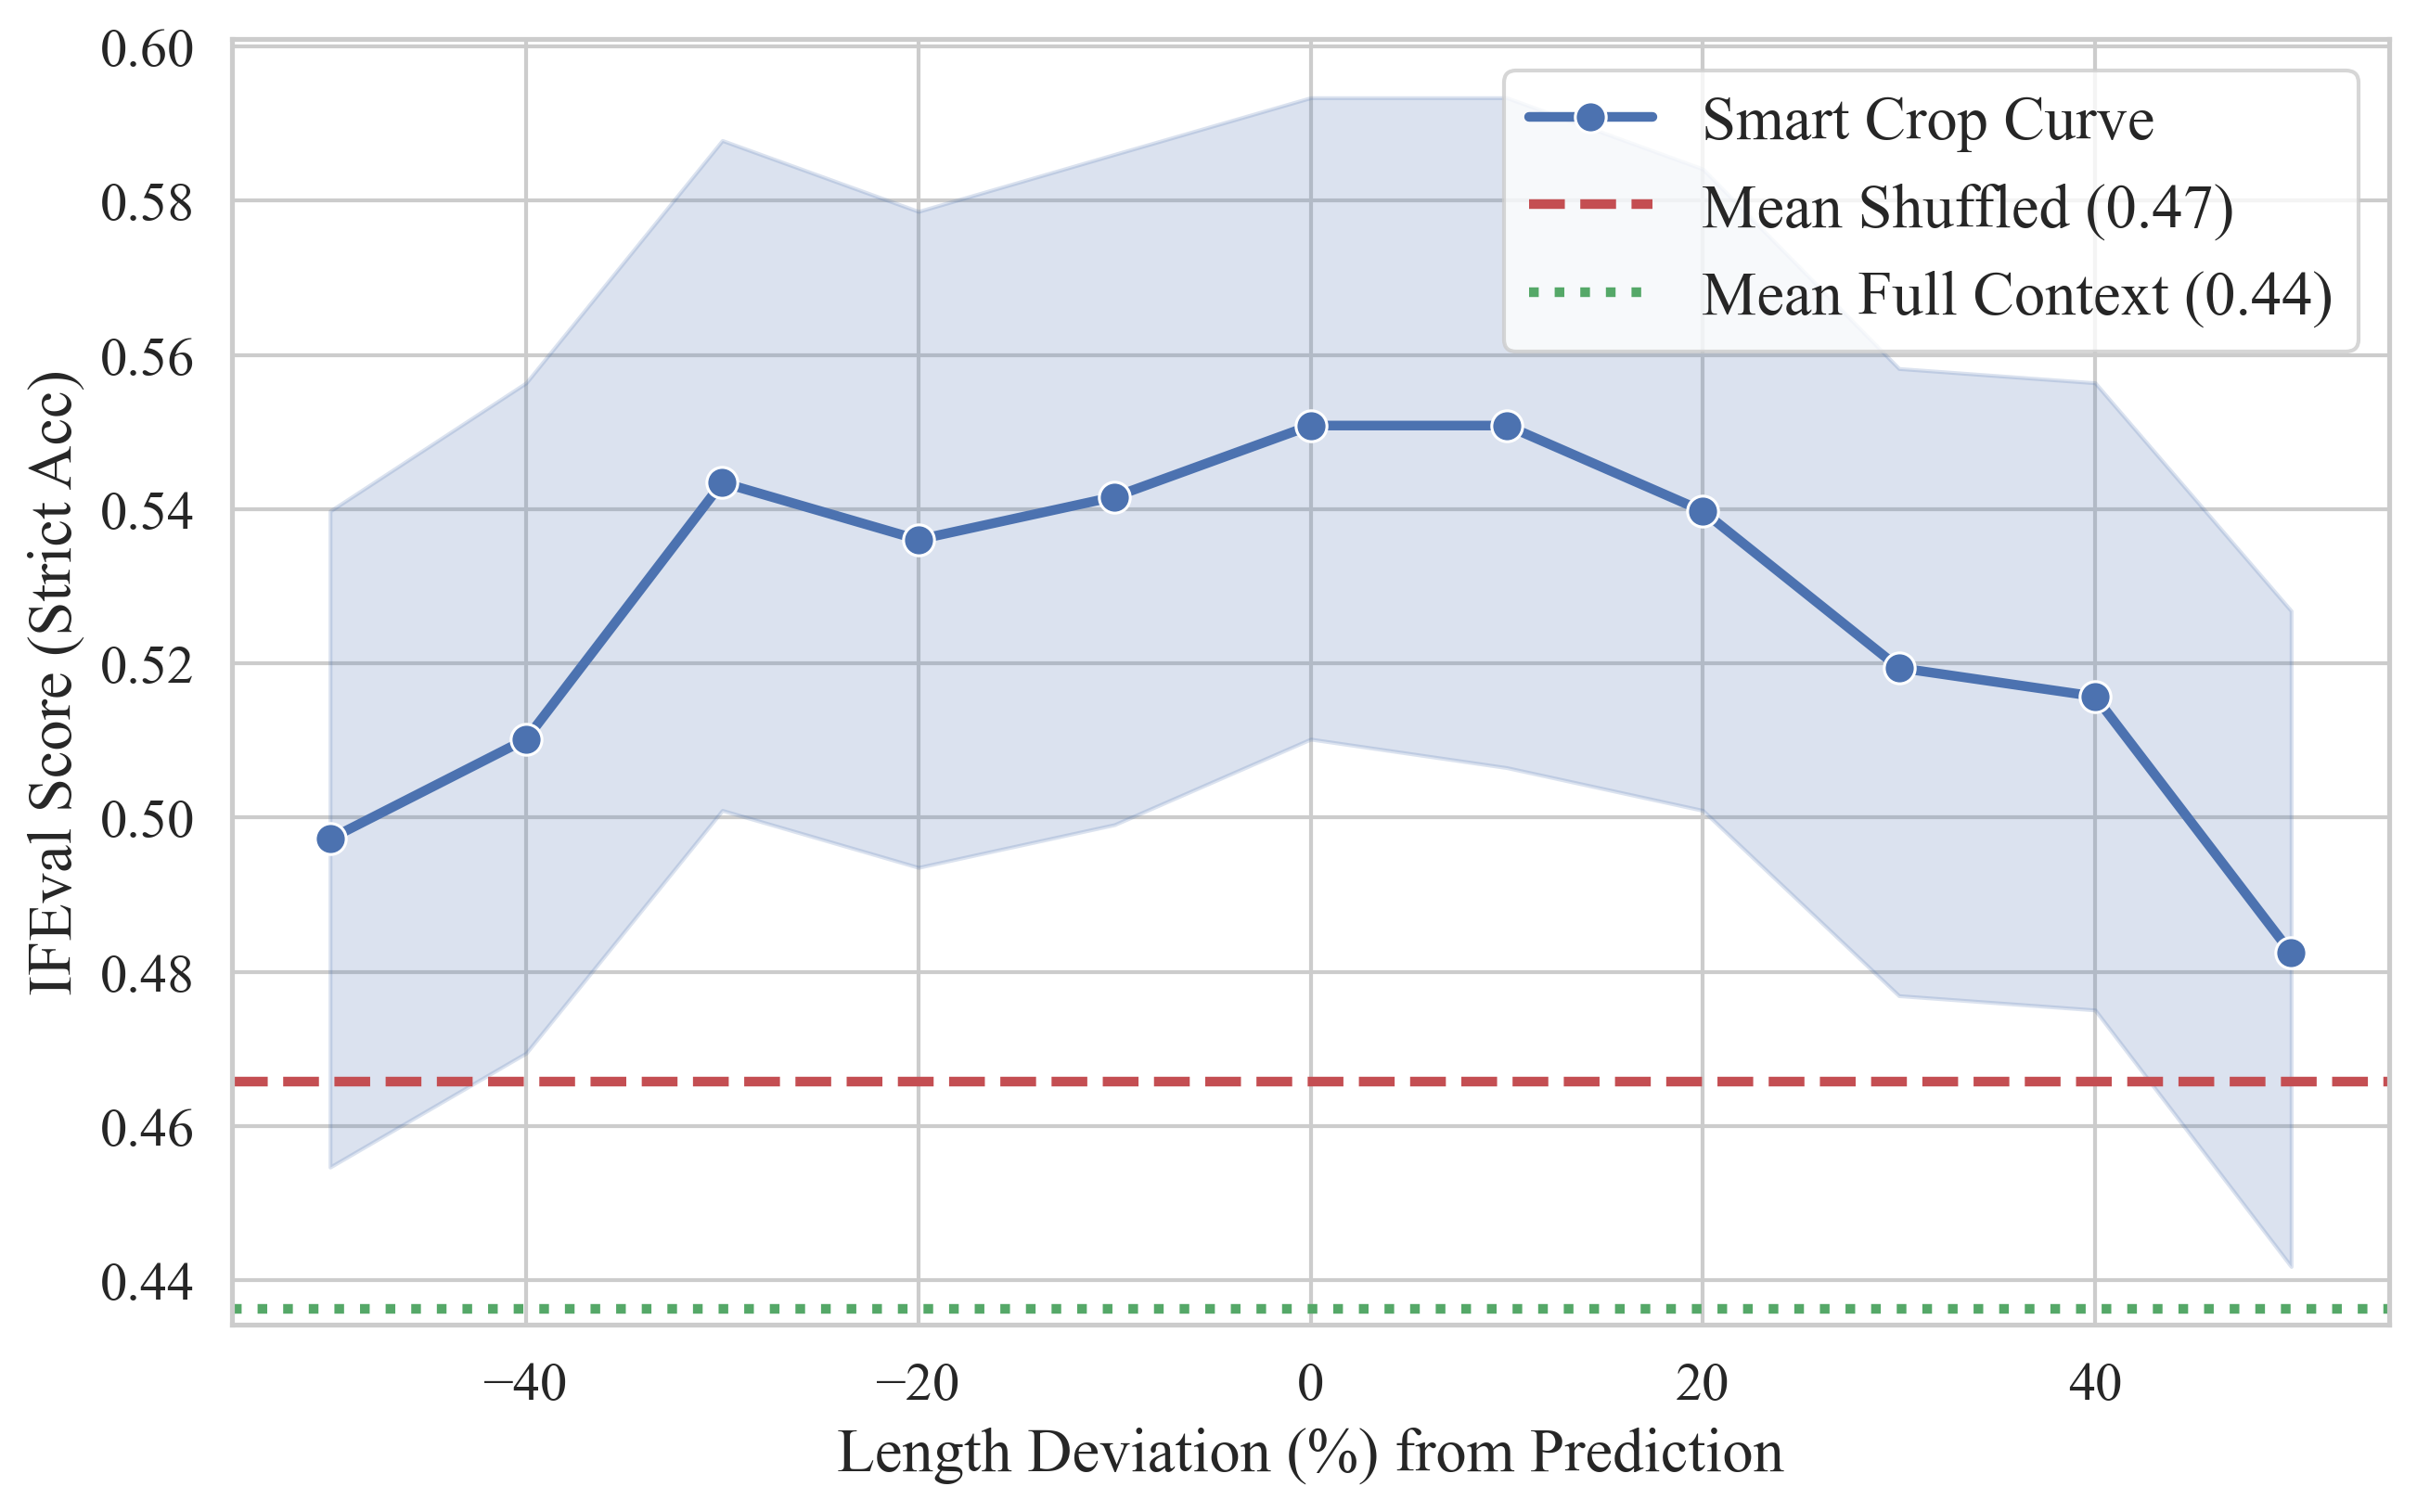
\includegraphics[width=\linewidth]{img/quality_length_sweep.png}
    \caption{\textbf{Sensitivity of \texttt{IfEval} Performance to Context Length Perturbations.} We analyze the robustness of \textsc{SmartCrop} by shifting the predicted length $\hat{L}$ by a deviation factor $\delta \in [-50\%, +50\%]$. The \textit{blue curve} shows the model performance (mean $\pm$ 95\% CI) across these varying context lengths. The \textit{red line} denotes the control baseline, where lengths are sampled from the empirical length distribution of other benchmarks. The \textit{green line} represents the \textit{Full Context} baseline performance. While the model is relatively robust to moderate under-estimation (negative $\delta$), generation quality degrades as superfluous padding is reintroduced (positive $\delta$), eventually converging toward the baseline.}
    \label{fig:quality_sweep}
\end{figure}


\section{Conclusion \& Discussion}
\label{sec:conclusion}

DLMs typically operate on a fixed-length canvas, employing special \texttt{EoS} tokens as padding to accommodate variable-length sequences. While this design simplifies the training and sampling pipeline, it imposes a significant ``padding tax'' at inference time: the model must process the entire context window even when the majority of the sequence consists of redundant placeholder tokens. In this work, we demonstrate that this computational overhead can be avoided. 

Specifically, we hypothesize that DLMs trained under the \texttt{EoS} paradigm, exemplified by the 8B-parameter \texttt{LLaDA} model, encode a usable length signal within the prompt's latent representation prior to the initiation of the denoising process. 

To exploit this latent signal, we introduce \textsc{SmartCrop}, a zero-shot, architecture-agnostic method. \textsc{SmartCrop} extracts this information by transforming the initial \texttt{EoS} logits into an inverse survival probability function across sequence positions, thereby estimating the probability of sequence termination at each token index. The method identifies the optimal truncation point as the first position where this probability exceeds a predefined threshold, enabling standard diffusion decoding on a significantly shorter canvas. Critically, \textsc{SmartCrop} requires no retraining, architectural modifications, or changes to the underlying decoder.

Our empirical evaluation confirms that \textsc{SmartCrop}, at many different probability thresholds, effectively predicts required output lengths and yields substantial efficiency gains across diverse benchmarks. Remarkably, this reduction in computation does not compromise model performance. In fact, we observe statistically significant performance improvements in two out of four tasks, with no degradation in the remaining two. These results suggest that excessive padding is not merely computationally wasteful but potentially detrimental; it may destabilize the denoising process by encouraging degenerate behavior in empty regions of the canvas. By constraining the generation space, \textsc{SmartCrop} shifts the model into a regime that favors more focused, higher-fidelity outputs.

Our sensitivity analysis further clarifies the nature of this length awareness. The distinct predicted length distributions across benchmarks indicate that the model internalizes task-specific priors, while the superior performance over shuffled controls points to a sophisticated, prompt-conditioned understanding of length. These findings suggest that length awareness is an emergent capability of DLMs trained with \texttt{EoS} padding, offering a promising path toward more efficient and robust non-autoregressive generation.

--
Our sensitivity analysis further elucidates the nature of this length awareness. The distinct predicted length distributions observed across benchmarks indicate that the model internalizes task-specific priors. Furthermore, the superior performance of \textsc{SmartCrop} relative to shuffled controls suggests a sophisticated, prompt-conditioned understanding of sequence length. These findings indicate that length awareness is an emergent capability of DLMs trained with \texttt{EoS} padding, offering a promising trajectory toward more efficient and robust non-autoregressive generation.

\paragraph{Limitations}
We report three main limitations.
First, \textsc{SmartCrop} complicates batch inference.
Different prompts lead to different cropped lengths preventing batch inference, unless the system groups requests by predicted length.
Second, our study covers one diffusion architectures and four English benchmarks.
The length signal may behave differently in other languages, domains, or decoding settings.
Third, \textsc{SmartCrop} relies on the model learning a meaningful \texttt{EoS} geometry.
Models with weak \texttt{EoS} calibration or no \texttt{EoS} in the vocabulary require further study.

\paragraph{Future work}
Several directions follow naturally.
The most interesting to us is to run the same length prediction at later denoising steps, as we expect that the accuracy increases as the denoising proceeds. However, this reduces the efficiency gains we observed.
Another direction would be to replace the heuristic quantile rule with a lightweight learned predictor that maps early latent states to a length distribution.
Lastly, length awareness can be exploited beyond context-cropping. For example, it could also adapt the denoising schedule, allocate compute across regions of the canvas, or trigger early stopping when the model has already converged, making diffusion decoding more adaptive.

\newpage

% In the unusual situation where you want a paper to appear in the
% references without citing it in the main text, use \nocite
\nocite{langley00}

\bibliography{main}
\bibliographystyle{icml2026}

%%%%%%%%%%%%%%%%%%%%%%%%%%%%%%%%%%%%%%%%%%%%%%%%%%%%%%%%%%%%%%%%%%%%%%%%%%%%%%%
%%%%%%%%%%%%%%%%%%%%%%%%%%%%%%%%%%%%%%%%%%%%%%%%%%%%%%%%%%%%%%%%%%%%%%%%%%%%%%%
% APPENDIX
%%%%%%%%%%%%%%%%%%%%%%%%%%%%%%%%%%%%%%%%%%%%%%%%%%%%%%%%%%%%%%%%%%%%%%%%%%%%%%%
%%%%%%%%%%%%%%%%%%%%%%%%%%%%%%%%%%%%%%%%%%%%%%%%%%%%%%%%%%%%%%%%%%%%%%%%%%%%%%%
\newpage
\appendix
\onecolumn
\section{Appendix}
\label{sec:appendix}



\end{document}